\section{Lecture 1}

\subsection{Signal and Noise}

\subsubsection{Material Reference}

The material in this lecture is primarily based on:

\textbf{TSE Book}
\begin{itemize}
    \item Chapter 1 (Sections 1.1 and 1.2): Overview of wireless communication
    \item Appendix A.1: Gaussian random variables
    \item Appendix A.2: Signal detection in Gaussian noise
\end{itemize}

\textbf{Haykin}
\begin{itemize}
    \item Chapter 2.2 (pp. 8--14)
    \item Chapter 2.8 (pp. 47--55)
\end{itemize}

This lecture establishes the physical and mathematical foundations required for analyzing wireless communication systems.

%------------------------------------------------
\subsection{Fundamental Quantities and Signal Representation}

Wireless communication systems operate by transmitting electrical signals that carry information. Two fundamental physical quantities describe these signals:

\textbf{Voltage} is the electrical potential difference (measured in volts), while  
\textbf{Power} is the rate at which energy is transferred (measured in watts).

In a resistive system with resistance $R$, instantaneous power is

\[
P(t) = \frac{v^2(t)}{R}.
\]

Because power depends on the square of voltage, small voltage variations can produce large power differences. This quadratic relationship is one reason why wireless systems are analyzed primarily in terms of power rather than voltage.

Wireless signals operate at high frequencies, ranging from kilohertz to gigahertz. Higher frequencies allow:
\begin{itemize}
    \item Higher data rates
    \item Smaller antenna sizes
    \item Greater available bandwidth
\end{itemize}

However, high frequencies also suffer from:
\begin{itemize}
    \item Increased path loss
    \item Stronger attenuation
    \item Greater susceptibility to noise
\end{itemize}

Therefore, the \textbf{signal-to-noise ratio (SNR)} becomes a central performance metric:

\[
\text{SNR} = \frac{P_s}{P_n}.
\]

%------------------------------------------------
\subsection{Noise and the AWGN Model}

In any realistic wireless system, the received signal is corrupted by noise. The most important noise source is thermal noise, generated by random electron motion in conductors.

Thermal noise is accurately modeled as \textbf{Additive White Gaussian Noise (AWGN)}.

It is:
\begin{itemize}
    \item \textbf{Additive} – it adds to the signal
    \item \textbf{White} – constant power spectral density
    \item \textbf{Gaussian} – normally distributed amplitude
\end{itemize}

The received signal model becomes:

\[
y(t) = x(t) + n(t).
\]

This simple model underpins almost all digital communication theory.

%------------------------------------------------
\subsection{Power in dBm and Logarithmic Representation}

Because wireless power levels span many orders of magnitude, logarithmic units are used.

Absolute power in dBm:

\[
P_{\mathrm{dBm}} = 10 \log_{10}\left(\frac{P}{1\,\mathrm{mW}}\right).
\]

Power ratios are expressed in dB:

\[
G_{\mathrm{dB}} = 10 \log_{10}\left(\frac{P_{\text{out}}}{P_{\text{in}}}\right).
\]

Important distinction:

\begin{itemize}
    \item dB → ratio
    \item dBm → absolute power
\end{itemize}

Logarithmic representation simplifies link budget calculations because gains and losses can be added directly.

%------------------------------------------------
\subsection{Logarithmic Identities}

Wireless analysis frequently requires converting between linear and logarithmic domains.

\[
\log_{10}(ab) = \log_{10}(a) + \log_{10}(b)
\]

\[
\log_{10}\left(\frac{a}{b}\right) = \log_{10}(a) - \log_{10}(b)
\]

\[
\log_{10}(a^n) = n \log_{10}(a)
\]

For information theory:

\[
\log_2(ab) = \log_2(a) + \log_2(b)
\]

Base-2 logarithms naturally arise when measuring information in bits.

%------------------------------------------------
\subsection{Signal Composition and Spectral Interpretation}

Signals may consist of multiple sinusoidal components. For example:

\[
x(t) = 2\sin(t) + \sin(5t).
\]

This represents a superposition of two frequency components. According to Fourier theory, any physically realizable signal can be decomposed into sinusoids.

This decomposition allows:
\begin{itemize}
    \item Frequency-domain analysis
    \item Filter design
    \item Bandwidth estimation
\end{itemize}

%------------------------------------------------
\subsection{Filters and Frequency Selectivity}

Filters shape signals in the frequency domain.

A low-pass filter allows frequencies below a cutoff frequency to pass.

\begin{figure}[h]
\centering
\begin{tikzpicture}
\begin{axis}[
    width=10cm,
    height=5cm,
    xlabel={Frequency},
    ylabel={Magnitude},
    ymin=0, ymax=1.1,
    domain=0:10,
    samples=200,
    axis lines=left
]
\addplot[thick] {1/(1 + exp(3*(x-4)))};
\end{axis}
\end{tikzpicture}
\caption{Low-pass filter magnitude response}
\end{figure}

A high-pass filter allows frequencies above the cutoff frequency.

\begin{figure}[h]
\centering
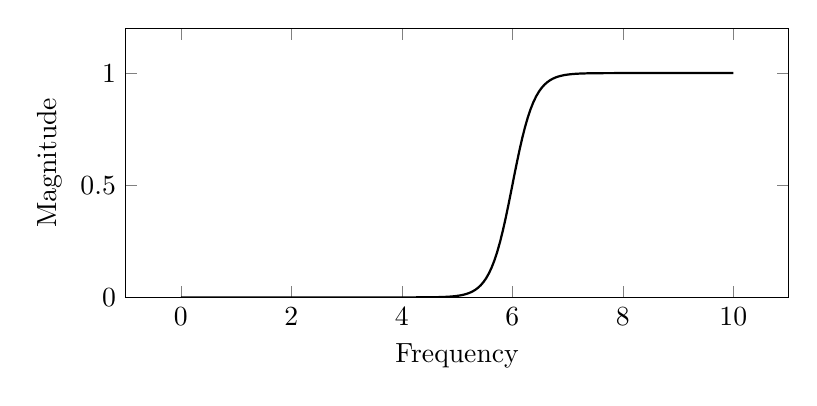
\begin{tikzpicture}
\begin{axis}[
    width=10cm,
    height=5cm,
    xlabel={Frequency},
    ylabel={Magnitude},
    ymin=0, ymax=1.2,
    domain=0:10,
    samples=200
]
\addplot[thick] {1/(1+exp(-5*(x-6)))}; 
\end{axis}
\end{tikzpicture}
\caption{High-pass filter magnitude response}
\end{figure}

Band-pass and notch filters similarly allow or suppress selected frequency regions.

%------------------------------------------------
\subsection{Link Budget Analysis}

A link budget accounts for all gains and losses between transmitter and receiver:

\[
P_{\mathrm{rx}} = P_{\mathrm{tx}} + G_{\mathrm{tx}} + G_{\mathrm{rx}} - L_{\mathrm{path}} - L_{\mathrm{other}}.
\]

All terms must be expressed consistently in dB or dBm.

This equation allows prediction of whether a communication link will close.

%------------------------------------------------
\subsection{Thermal Noise, Temperature, and Bandwidth}

Thermal noise power in linear units:

\[
P_n = k_B T B
\]

where:
\begin{itemize}
    \item $k_B$ = Boltzmann constant
    \item $T$ = absolute temperature
    \item $B$ = bandwidth
\end{itemize}

At room temperature:

\[
N_0 \approx -174 \text{ dBm/Hz}.
\]

Total noise power:

\[
P_n = -174 + 10\log_{10}(B).
\]

Increasing bandwidth increases noise power linearly.

%------------------------------------------------
\subsection{Shannon Capacity and Fundamental Limits}

The maximum achievable data rate is:

\[
C = B \log_2(1 + \gamma),
\]

where

\[
\gamma = \frac{P_s}{P_n}.
\]

Key insight:

Capacity increases logarithmically with SNR. Doubling power does not double capacity.

\begin{figure}[h]
\centering
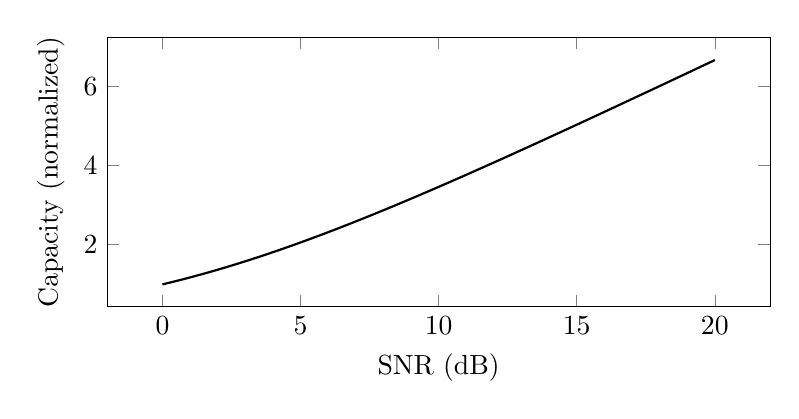
\begin{tikzpicture}
\begin{axis}[
    width=10cm,
    height=5cm,
    xlabel={SNR (dB)},
    ylabel={Capacity (normalized)},
    domain=0:20,
    samples=200
]
\addplot[thick] {ln(1 + 10^(x/10))/ln(2)};
\end{axis}
\end{tikzpicture}
\caption{Logarithmic growth of capacity with SNR}
\end{figure}

%------------------------------------------------
\subsection{Energy per Bit and BER}

Digital systems are commonly analyzed using:

\[
\frac{E_b}{N_0}
\]

where:
\begin{itemize}
    \item $E_b$ = energy per bit
    \item $N_0$ = noise spectral density
\end{itemize}

The \textbf{Bit Error Rate (BER)} is the probability that a transmitted bit is incorrectly detected.

Higher $E_b/N_0$ reduces BER.

This metric allows comparison of modulation schemes independent of bandwidth.
